% proposed method ---
\chapter[Active Period Detection Method of Primary Signal for Spectrum Database]{Proposed Method}
\label{chapter:Propose}
\section{System model}
\label{system}

We assume that a sensor node tunes to a frequency band and obtains samples ${\bf y}=\left\{y[1],y[2],...,y[N]\right\}$ from a primary transmitter. $N$ is the sample number during the sensing period. Since a multiple ON/OFF environment is considered, the sensing samples ${\boldmath y}$ is shown in Fig. 2 as follows

\begin{eqnarray}
y[i] = 
\begin{cases}
\;n[i],    i=1,...\tau_1-1 \\ \nonumber
\; \\ \nonumber
\;x[i]+n[i], i=\tau_1,...,\tau_2-1 \\
\; \\ \nonumber
\;n[i],    i=\tau_2,..,N,
\end{cases}
\end{eqnarray}

where $\tau_1$ and $\tau_2$ is the rise up point at which primary user starts to transmit and rise down point at which primary user stop transmitting respectively. If $\tau_1=1$ and $\tau_2=N$, the primary user is always transmitting during the sensing period. On the other hand, if $\tau_1=1$ and $\tau_2=1$, the primary user is not at present during the sensing period. In this paper, we consider only the primary user starts and stops transmission during the sensing period.
If the primary user is not transmitting, $y[i] = n[i]$, in which $n[i]$ is Addative White Gaussian Noise with mean 0 and variance $\sigma^2$. If the primary user starts transmitting, then $y[i] = x[i] + n[i]$, in which $x[i] = gs[i]$. $g$ is the channel gain and the $s[i]$ is the signal of the primary user. Therefore, we assume $x[i]$ is white and Gaussian with mean 0 and variance $P$. $P$ depends on the channel gain and the transmitter power of the primary user. In the wireless environment, the signal of the primary experiences pathloss and shadowing and  multipath fading, so the value of $P$ is not possible to be known accurately by the sensor. Thus, as a solution to received power detection problem, a transition point detection algorithm is considered. 

\section{Transition Point Detection Method under Multiple ON/OFF Environment }    

In this section, transition point detection algorithm for the status of primary user is introduced in detail. As the Fig. \ref{system_model} is shown, the sample of the ON and OFF status follows a Gaussian distribution $\mathcal{N}(0,\sigma^2+P)$ and $\mathcal{N}(0,\sigma^2)$ respectively. The probability density function(PDF) follows the eq. (\ref{normal}) is given by

\begin{eqnarray}
\begin{cases}
\;f_0(t) = \frac{1}{\sqrt{2\pi\sigma^2}} \rm{exp}^{-\frac{t^2}{2\sigma^2}} \\
\; \\ \nonumber
\;f_1(t) = \frac{1}{\sqrt{2\pi(\sigma^2+P)}} \rm{exp}^{-\frac{t^2}{2(\sigma^2+P)}}.
\end{cases}
\label{normal}
\end{eqnarray}

\begin{center}
  \begin{figure}[t]
    \centering
    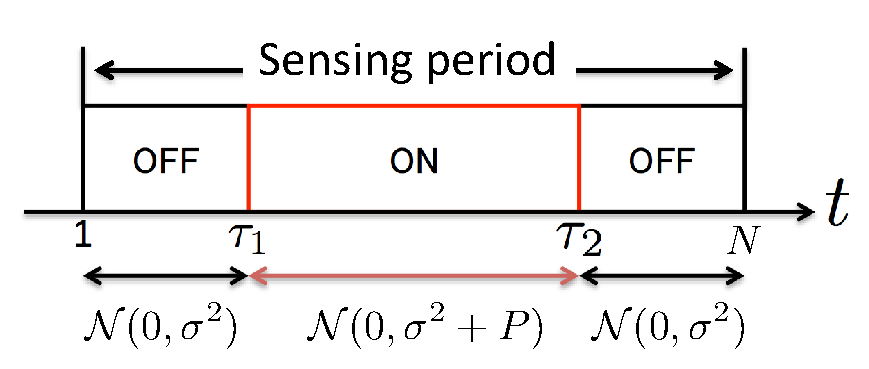
\includegraphics[width=90mm]{systemodel.eps}
    \label{system_model}
    \caption{\normalsize{System model.}}
  \end{figure}
\end{center} 

\subsection{CUSUM algorithm}
The cumulative sum (CUSUM) algorithm, which was first proposed by Page in \cite{ref:CUSUM}, is used to detection the transition point when $P$ and $\sigma^2$ is assumed to be known.
The PDF $f_0(t)$ and $f_1(t)$ are fully specified. Thus, the log probability density ratio $l(y[i])$ is also fully defined by the eq. (\ref{like1}) and (\ref{like2}),

\begin{eqnarray}
l_{0}(y[i]) &=& {\rm ln}\left\{\frac{f_0(y[i])}{f_1(y[i])}\right\} \label{like1} \\ 
&=& -\frac{2(P+\sigma^2)\sigma^2}{Py^2[i]} + \frac{1}{2}{\rm ln}\left\{\frac{P+\sigma^2}{\sigma^2}\right\}, \nonumber
\end{eqnarray}

\begin{eqnarray}
l_{1}(y[i]) &=& {\rm ln}\left\{\frac{f_1(y[i])}{f_0(y[i])}\right\} \label{like2} \\ 
&=& \frac{Py^2[i]}{2(P+\sigma^2)\sigma^2} + \frac{1}{2}{\rm ln}\left\{\frac{\sigma^2}{P+\sigma^2}\right\}. \nonumber
\end{eqnarray}

When the primary user is on the OFF and ON status, the average log probability density ratio can be calculated respectively using the eq. (\ref{D_f0}) and (\ref{D_f1}),
\begin{eqnarray}
E_{f_0}\left\{l_0(y[i])\right\} &=& -\int f_0(y){\rm ln}\left\{\frac{f_0(y)}{f_1(y)}\right\}dy \nonumber \\ 
&=&-D(f_0||f_1)\leq 0, \label{D_f0} 
\end{eqnarray}
\begin{eqnarray}
E_{f_1}\left\{l_1(y[i])\right\} &=& \int f_1(y){\rm ln}\left\{\frac{f_1(y)}{f_0(y)}\right\}dy \nonumber \\
&=& D(f_1||f_0)\geq 0 \label{D_f1},
\end{eqnarray}
where $D(f_0||f_1)$ is the Kullback-Leibler divergence of $f_0$ from $f_1$ and $D(f_1||f_0)$ vice versa, which is shown in eq. (\ref{KL})
\begin{eqnarray}
D(f_0||f_1)=\frac{P}{2(P+\sigma^2)}+\frac{1}{2}{\rm ln}\left\{\frac{\sigma^2}{\sigma^2+P}\right\}.
\label{KL}
\end{eqnarray}
Hence, when the primary user is at present, which means the sample before primary user changes its status from OFF to ON, the probability density ratio $l(y)$ has a negative trend. After a change point from ON to OFF, $l(y)$ has a positive trend.
Using the characterics discussed above, an algorithm for detecting a status transition (ON$\rightarrow$OFF or OFF$\rightarrow$ON) of the primary user can be defined as comparing,  
\begin{eqnarray}
g_t =  \max_{k \leq t}\left\{\sum_{i=1}^tl(y[i]-\sum_{i=1}^kl(y[i]))\right\}=\max_{k \leq t}\sum_{i=k+1}^tl(y[i]),
\label{Cusum}
\end{eqnarray}
with a threshold $h$. If $g_t$ is larger than $h$, the existence of the primary user is declared. Since $l(y)$ has a positive trend during the ON status of the primary.

\begin{figure}[t]
\centering
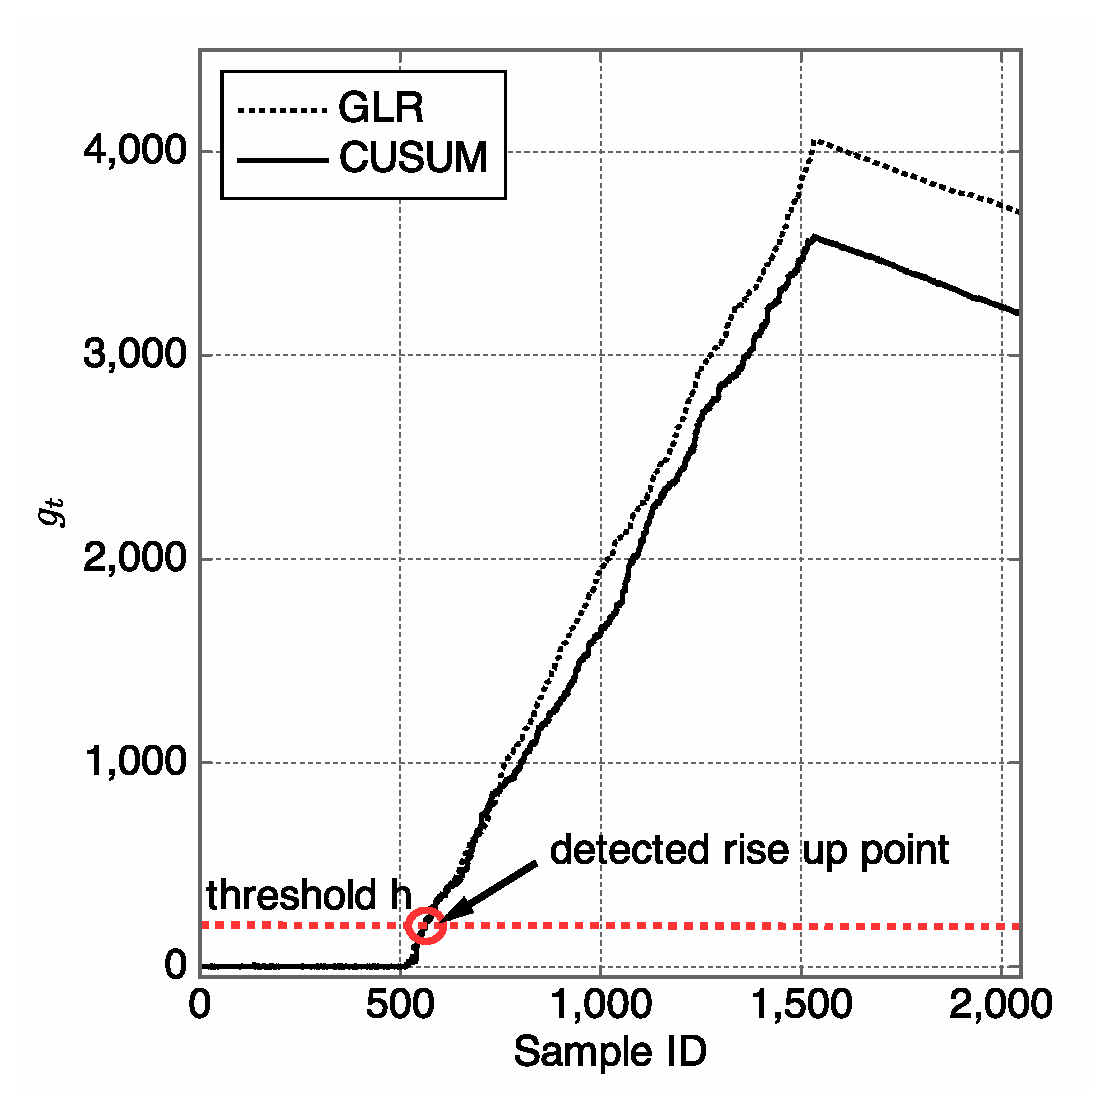
\includegraphics[width=87mm]{OFF2ON.eps}
\caption{ Statistic $g_t$ using the probability density ratio $l_0(y)$  when the rise up point is 512th sample and the rise down point is 1532th sample.}
\label{OFF2ON}
\end{figure}

Also, the eq. (\ref{Cusum}) can be written as
\begin{eqnarray}
g_{t+1} &=& \max_{k \leq t+1}\left\{\sum_{i=k+1}^{t+1}l(y[i])\right\} \nonumber \\ 
&=& \max\left\{\max_{k \leq t+1}\left\{\sum_{i=k+1}^{t+1}l(y[i])\right\},0\right\} \nonumber \\
&=& \max\left\{\max_{k \leq t+1}\left\{\sum_{i=k+1}^{t+1}l(y[i])\right\}+l(y[i]),0\right\} \nonumber \\
&=& \left\{g_t+l(y[t+1])\right\}^{+}.
\label{rec}
\end{eqnarray}
$\left\{.\right\}^{+}$means that the value must be postive. Hence, $g_t$ can be computed recursively by setting $g_0=0$. To sum up, the CUSUM algorithm works as the following process:
\begin{enumerate}
  \item[i]. compute $l(y)$ for each sample using eq. (\ref{like1}) or (\ref{like2}).
  \item[ii]. compute the statistic $g_t$ using eq. (\ref{rec}).
  \item[iii]. compare the statistic $g_t$ with a threshold $h$.
  \item[iv]. If $g_t \geq h$, the existence of the primary user is declared.
\end{enumerate}

\subsection{GLR algorithm}
In realistic wireless channels, the exact value of $P$ is difficult to be known exactly. It is more reasonable to assume that $P$ belongs to a range, that is $P\in[P_{{\rm min}}, P_{\rm {max}}]$. In this case, a generalized likelihood ratio(GLR) algorithm\cite{ref:GLR} for transition point detection is applied. Since the value of $P$ is unknown, the statistic $g_t$ is defined as the following eq. (\ref{Glr}),
\begin{eqnarray}
g_t &=& \max_{k \leq t}\left\{ \sum_{i=k+1}^tl(y[i])\right\}={\rm ln}\left\{\prod_{i=k+1}^k\frac{f_{1,P}(y[i])}{f_0(y[i])}\right\} \nonumber \\ 
   &=& \max_{k \leq t}\left\{\sum_{i=k+1}^t\left\{ \frac{Py^2[i]}{2(P+\sigma^2)\sigma^2}+\frac{1}{2} {\rm ln}(\frac{\sigma^2}{P+\sigma^2}) \right\}\right\},
\label{Glr}
\end{eqnarray}
\begin{figure}[t]
\centering
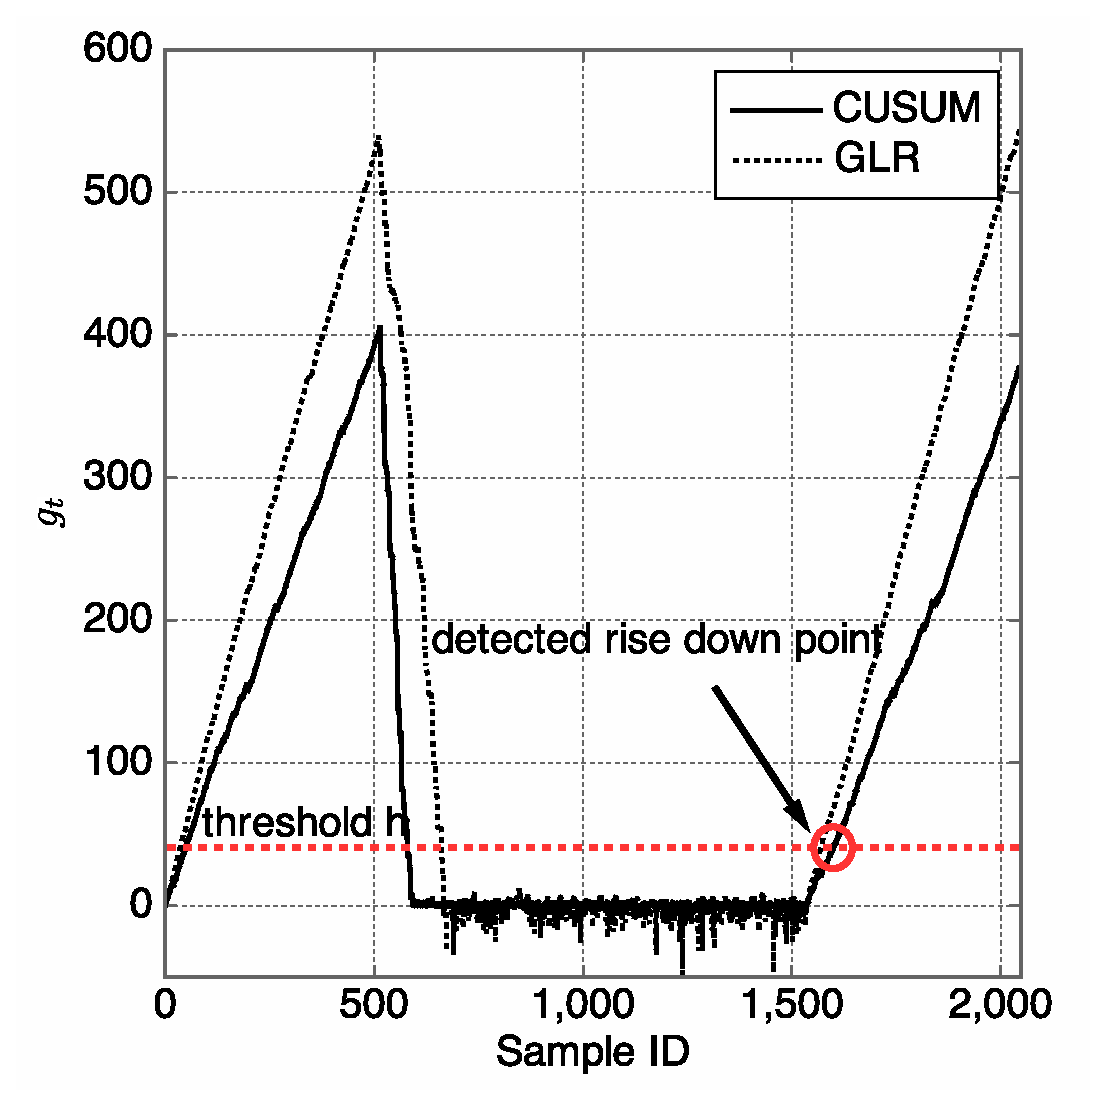
\includegraphics[width=87mm]{ON2OFF.eps}
\caption{Statistic $g_t$ using the probability density ratio $l_1(y)$ when the raise up point is 512th sample and the raise down point is 1532th sample.}
\label{ON2OFF}
\end{figure}
where $f_{1,P}(t)$ is the probability density function of the received signal when the varinace of the signal part is $P$. Therefore a function $f(P)$ defined as eq. (\ref{fp}) is used to calculate the statistic $g_t$,
\begin{eqnarray}
f(P) &=& \sum_{i=k+1}^t\left\{ \frac{Py^2[i]}{2(P+\sigma^2)\sigma^2}+\frac{1}{2} {\rm ln}(\frac{\sigma^2}{P+\sigma^2})\right\} \nonumber\\ 
&=&\frac{P}{2(P+\sigma^2)\sigma^2}\hat{y}+(t-k)\frac{1}{2}{\rm ln}\left\{ \frac{\sigma^2}{P+\sigma^2} \right\},
\label{fp}
\end{eqnarray}
where $\hat{y}=\sum_{i=k+1}^t y[i]$. To find a the power $P^{*}$ that maximizes the function $f(P)$ over $P \in [P_{{\rm min}}, P_{{\rm max}}]$, it can be calculated as below,

\begin{align}
P^{*}=
\begin{cases}
\;P_{{\rm max}}, & (t-k)\leq\frac{\hat{y}}{P_{{\rm max}}+\sigma^2}, \\
\; \\ 
\;\frac{\hat{y}}{t-k}-\sigma^2, & \frac{\hat{y}}{P_{{\rm max}}+\sigma^2}\leq(t-k)\leq\frac{\hat{y}}{P_{{\rm min}}+\sigma^2}, \label{maxP} \\ 
\; \\
\; P_{{\rm min}}, & (t-k) \geq \frac{\hat{y}}{P_{{\rm min}}+\sigma^2}.
\end{cases}
\end{align}

As same as the CUSUM algorithm, in the GLR algorithm the statistic value $g_t$ is calculated in eq.(\ref{Glr}) with choosing the a power $P^{*}$ from the eq.(\ref{maxP}), and is compared with the threshold $h$. Once $g_t>h$, the existance of the primary user is declared.

\subsection{Threshold configuration for CUSUM and GLR algorithm}
To set a threshold for the transition point detection, we first assume $t_0$ denotes the time when the statistic $g_t$ exceeds the threshold $h$, and define $\bar{T_0}=E[t_0]$ is the mean time to a false alarm. Following \cite{ref:threshold_cusum} and \cite{ref:threshold_GLR}, some simple bounds on $\bar{T_0}$ can be derived.

For CUSUM algorithm, the relationship between the mean false alarm and threshold is as follows.
\begin{eqnarray}
\bar{T_0} \geq e^h.
\end{eqnarray}
For GLR algorithm, the threshold is set to be $h=-{\rm ln}\left\{\frac{a}{b}\right\}$ , where 
\begin{eqnarray}
b=3{\rm ln}\left\{a^{-1}(1+\frac{1}{D(f_1,P_{min}||f_0)})^2\right\},
\end{eqnarray}
and $a$ follows the following inequality.
\begin{eqnarray}
\bar{T_0} \geq \frac{1}{a}.
\end{eqnarray}
